%%%%%%%%%%%%%%%%%%%%%%%%%%%%%%%%%%%%%%%%%%
%%%%%%%%%%%%%                 %%%%%%%%%%%%
%%%%%%%%%%%%%    EXERCISE 1   %%%%%%%%%%%%
%%%%%%%%%%%%%                 %%%%%%%%%%%%
%%%%%%%%%%%%%%%%%%%%%%%%%%%%%%%%%%%%%%%%%%
\begin{exercise}[]{ SMS, iMessage, and WhatsApp are all smartphone real-time messaging systems. After doing some research on the Internet, for each of these systems write one paragraph about the protocols they use. Then write a paragraph explaining how they differ. (10 points)
    }
  \begin{solution}
  \par{~}

  SMS (short message service) uses ``SMPP''(simple mail transport protocol) protocol. The SMPP protocol\footnote{https://www.txt180.com/article/sms-v-smtp-text-message/} is developed by the telecommunications industry specifically for transmitting SMS messages. SMPP is the protocol used whenever a text message is sent from a mobile phone to another mobile phone. It is simple and compact, which saves bandwidth. SMPP provides full 2 way communications between phones and applications.

  iMessage is only used for Apple devices. The iMessage protocol\footnote{https://en.wikipedia.org/wiki/IMessage} is based on the Apple Push Notification service (APNs)—a proprietary, binary protocol. It sets up a Keep-Alive connection with the Apple servers. Every connection has its own unique code, which acts as an identifier for the route that should be used to send a message to a specific device. The connection is encrypted with TLS using a client-side certificate, that is requested by the device on the activation of iMessage.

  WhatsApp Messenger, or simply WhatsApp, is an American freeware, cross-platform centralized messaging and voice-over-IP (VoIP) service owned by Facebook, Inc. WhatsApp uses a customized version of the open standard Extensible Messaging and Presence Protocol (XMPP)\footnote{https://en.wikipedia.org/wiki/XMPP}. Based on XML (Extensible Markup Language), it enables the near-real-time exchange of structured data between any two or more network entities. XMPP is defined in an open standard in the application layer. The architecture of the XMPP network is similar to email; anyone can run their own XMPP server and there is no central master server. This federated open system approach allows users to interoperate with others on any server using a `JID' user account, similar to an email address.




  APNs is closed source, limited to Apple devices and a proprietary protocol, while SMPP and XMPP are open and portable to various devices. SMPP can only be used to deliver text messages with limited length, while APNs and XMPP support flexible contents. SMPP is not encrypted while APNs and XMPP are encrypted.
  \end{solution}
  \label{ex1}
\end{exercise}


%%%%%%%%%%%%%%%%%%%%%%%%%%%%%%%%%%%%%%%%%%
%%%%%%%%%%%%%                 %%%%%%%%%%%%
%%%%%%%%%%%%%    EXERCISE 2   %%%%%%%%%%%%
%%%%%%%%%%%%%                 %%%%%%%%%%%%
%%%%%%%%%%%%%%%%%%%%%%%%%%%%%%%%%%%%%%%%%%
\begin{exercise}[]{Consider an HTTP client that wants to retrieve a Web document at a given URL. The IP address of the HTTP server is initially unknown. What transport and application-layer protocols besides HTTP are needed in this scenario? (10 points)}
  \begin{solution}
  \par{~}
  \begin{enumerate}
      \item Application Layer:  DNS for looking up the IP address of the server
      \item Transport layer: UDP for DNS service
      \item Transport layer: TCP for HTTP service
  \end{enumerate}
  \end{solution}
  \label{ex2}
\end{exercise}


%%%%%%%%%%%%%%%%%%%%%%%%%%%%%%%%%%%%%%%%%%
%%%%%%%%%%%%%                 %%%%%%%%%%%%
%%%%%%%%%%%%%    EXERCISE 3   %%%%%%%%%%%%
%%%%%%%%%%%%%                 %%%%%%%%%%%%
%%%%%%%%%%%%%%%%%%%%%%%%%%%%%%%%%%%%%%%%%%
\begin{exercise}[]{The text below in figure \ref{fig:1} shows the reply sent from the server in response to the HTTP GET message in the question above. Answer the following questions, indicating where in the message below you find the answer.(20 points)

    \begin{figure}[hb]
        \begin{center}
        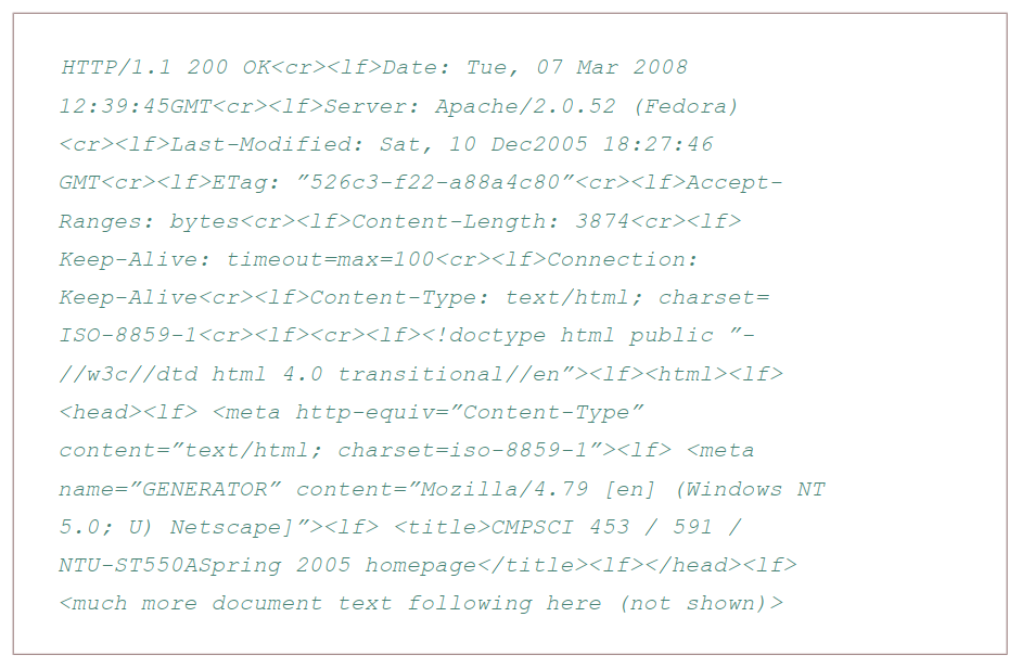
\includegraphics[width=12cm]{img/ass2/hw2_1}
        \caption{The text in P3}
        \label{fig:1}
        \end{center}
      \end{figure}
    \begin{enumerate}
        \item Was the server able to successfully find the document or not? What time was the document reply provided? (5 points)
        \item When was the document last modified? (5 points)
        \item  How many bytes are there in the document being returned? (5 points)
        \item What are the first 5 bytes of the document being returned? Did the server agree to a persistent connection? (5 points)
    \end{enumerate}
    }
  \begin{solution}
  \par{~}
  \begin{enumerate}
      \item The server was able to locate the document successfully, since the status code is 200. The reply was provided on Tuesday, 07 Mar 2008 12:39:45 GMT.
      \item The document was last modified on Saturday 10 Dec 2005 18:27:46 GMT.
      \item There are 3874 bytes in the document being returned.
      \item First five bytes \texttt{<!doc}. The server agreed with a persistent connection from \texttt{Connection: Keep-alive} field.
  \end{enumerate}
  \end{solution}
  \label{ex3}
\end{exercise}


%%%%%%%%%%%%%%%%%%%%%%%%%%%%%%%%%%%%%%%%%%
%%%%%%%%%%%%%                 %%%%%%%%%%%%
%%%%%%%%%%%%%    EXERCISE 4   %%%%%%%%%%%%
%%%%%%%%%%%%%                 %%%%%%%%%%%%
%%%%%%%%%%%%%%%%%%%%%%%%%%%%%%%%%%%%%%%%%%
\begin{exercise}[]{Suppose within your Web browser you click on a link to obtain a Web page. The IP address for the associated URL is not cached in your local host, so a DNS lookup is necessary to obtain the IP address. Suppose that n DNS servers are visited before your host receives the IP address from DNS; the successive visits incur an RTT of RTT1, ..., RTTn. Further suppose that the Web page associated with the link contains exactly one object, consisting of a small amount of HTML text. Let RTT0 denote the RTT between the local host and the server containing the object. Assuming zero transmission time of the object, how much time elapses from when the client clicks on the link until the client receives the object?
    
    }
  \begin{solution}
  \par{~}
  The total amount of time to get the IP address is: $RTT_{1}+RTT_{2}+\ldots+RTT_{\mathrm{n}}$

  The total response time is DNS elapsing time plus RTT for TCP request and receive the small object. 
    $2 RTT_{0}+RTT_{1}+RTT_{2}+\ldots+RTT_{\mathrm{n}}$
  \end{solution}
  \label{ex4}
\end{exercise}


%%%%%%%%%%%%%%%%%%%%%%%%%%%%%%%%%%%%%%%%%%
%%%%%%%%%%%%%                 %%%%%%%%%%%%
%%%%%%%%%%%%%    EXERCISE 5   %%%%%%%%%%%%
%%%%%%%%%%%%%                 %%%%%%%%%%%%
%%%%%%%%%%%%%%%%%%%%%%%%%%%%%%%%%%%%%%%%%%
\begin{exercise}[]{Referring to Problem \ref{ex4}, suppose the HTML file references eight very small objects on the same server. Neglecting transmission times, how much time elapses with (15 points)

    1. Non-persistent HTTP with no parallel TCP connections? (5 points)

    2. Non-persistent HTTP with the browser configured for 5 parallel connections? (5 points) 
    
    3. Persistent HTTP? (5 points)}
  \begin{solution}
  \par{~}
  \begin{enumerate}
      \item Elapsing time =  DNS lookup + transmit HTML + transmit 8 files = $RTT_{1}+RTT_{2}+\ldots+RTT_{\mathrm{n}} +2 RTT_{0} + 8 \times 2 RTT_{0} = RTT_{1}+RTT_{2}+\ldots+RTT_{\mathrm{n}} + 18 RTT_{0} $
      \item Elapsing time =  DNS lookup + transmit HTML + transmit in two phases $(2\times 5 > 8)$ = $RTT_{1}+RTT_{2}+\ldots+RTT_{\mathrm{n}} + 2 RTT_{0} + 2 \times 2 RTT_{0} = RTT_{1}+RTT_{2}+\ldots+RTT_{\mathrm{n}} + 6 RTT_{0} $
      \item If without pipelining, Elapsing time =  DNS lookup + transmit HTML + transmit 8 files $RTT_{1}+RTT_{2}+\ldots+RTT_{\mathrm{n}} + 2 RTT_{0} + 8 RTT_{0} = RTT_{1}+RTT_{2}+\ldots+RTT_{\mathrm{n}} + 10 RTT_{0} $
      
      If with pipelining, Elapsing time =  DNS lookup + transmit HTML + transmit 8 files together $RTT_{1}+RTT_{2}+\ldots+RTT_{\mathrm{n}} + 2 RTT_{0} + RTT_{0} = RTT_{1}+RTT_{2}+\ldots+RTT_{\mathrm{n}} + 3 RTT_{0} $
  \end{enumerate}
  \end{solution}
  \label{ex5}
\end{exercise}


%%%%%%%%%%%%%%%%%%%%%%%%%%%%%%%%%%%%%%%%%%
%%%%%%%%%%%%%                 %%%%%%%%%%%%
%%%%%%%%%%%%%    EXERCISE 6   %%%%%%%%%%%%
%%%%%%%%%%%%%                 %%%%%%%%%%%%
%%%%%%%%%%%%%%%%%%%%%%%%%%%%%%%%%%%%%%%%%%
\begin{exercise}[]{Consider Figure \ref{fig:2} , for which there is an institutional network connected to the Internet. Suppose that the average object size is 850,000 bits and that the average request rate from the institution's browsers to the origin servers is 16 requests per second. Also suppose that the amount of time it takes from when the router on the Internet side of the access link forwards an HTTP request until it receives the response is three seconds on average (see Section 2.2.5). Model the total average response time as the sum of the average access delay (that is, the delay from Internet router to institution router) and the average Internet delay. For the average access delay, use $\Delta /(1-\Delta \beta)$ where $\Delta$ is the average time required to send an object over the access link and $\mathrm{b}$ is the arrival rate of objects to the access link (10 points)
\begin{figure}[hb]
  \begin{center}
  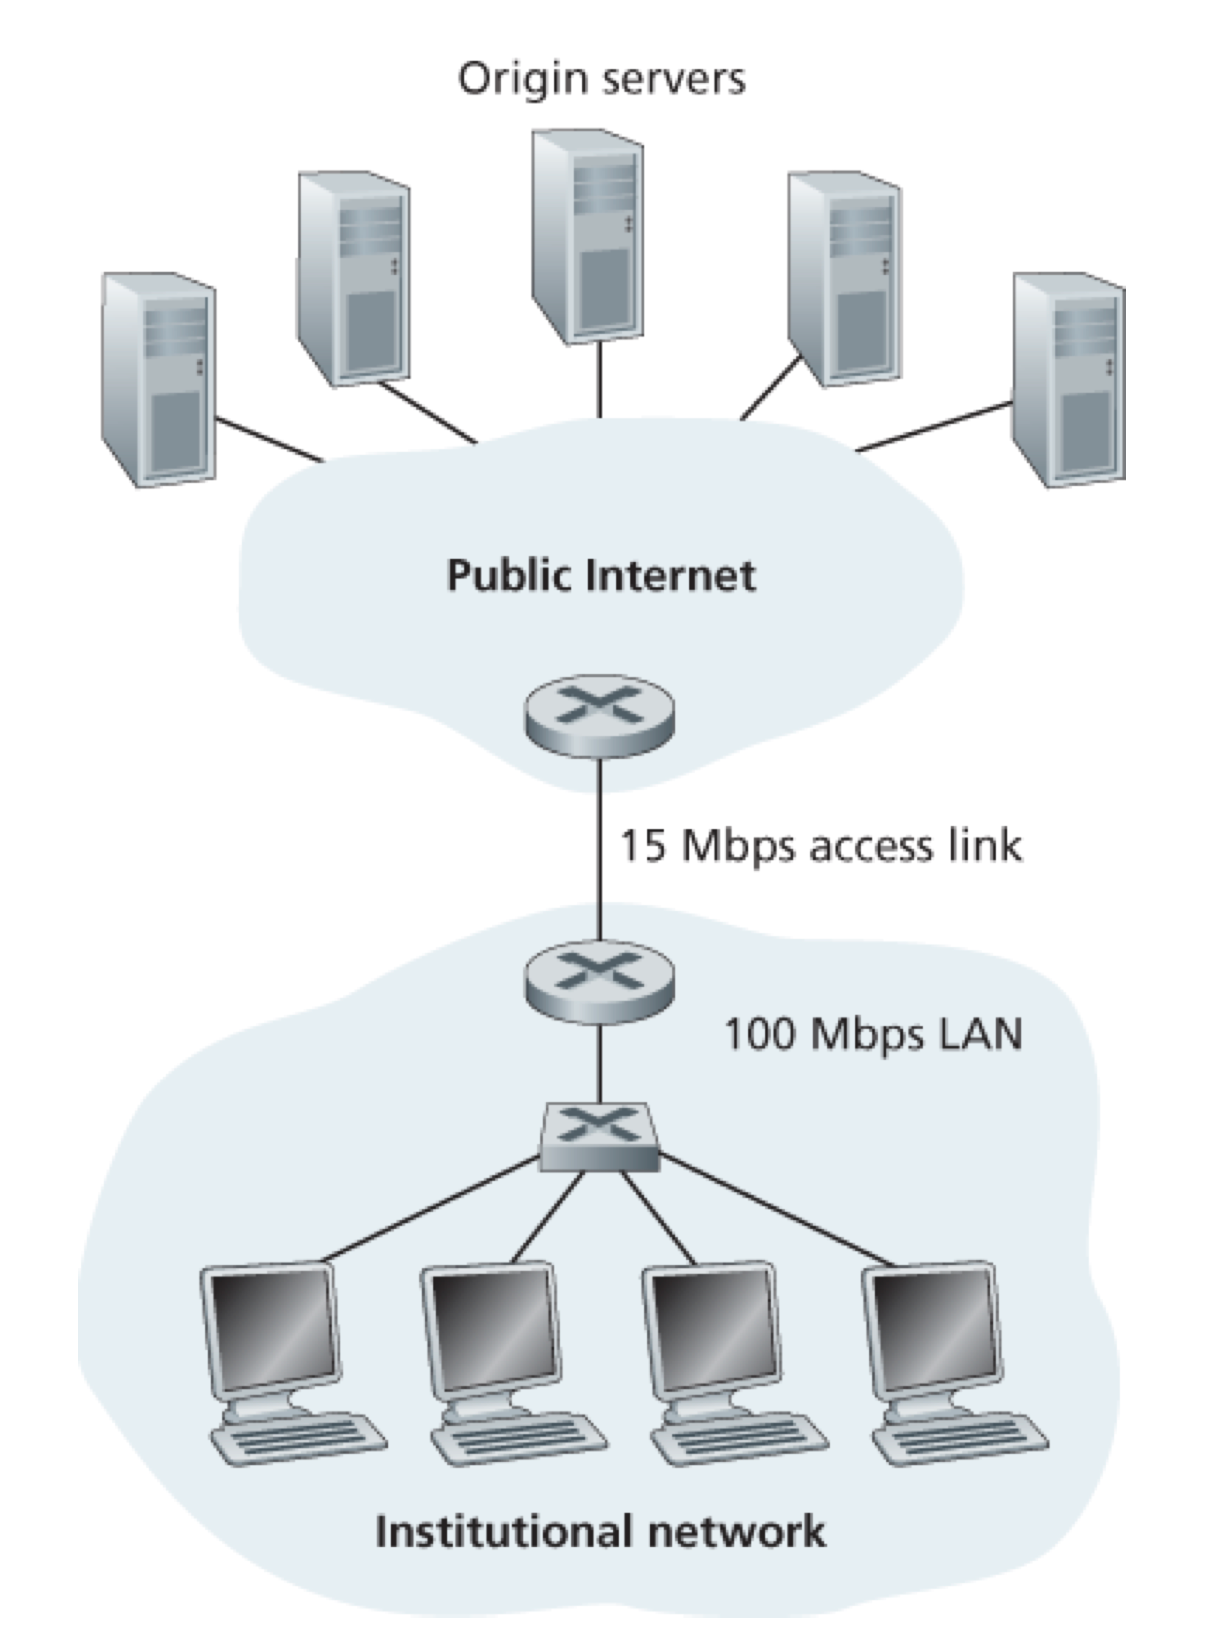
\includegraphics[width=12cm]{img/ass2/hw2_2}
  \caption{Bottleneck between an institutional network and the Internet}
  \label{fig:2}
  \end{center}
\end{figure}
    1. Find the total average response time. (5 points)

    2. Now suppose a cache is installed in the institutional LAN. Suppose the miss rate is 0.4. Find the total response time. (5 points)}
  \begin{solution}
  \par{~}
  \begin{enumerate}
      \item Transmission delay $\Delta = 850,000 / 150,000,000 = 0.0567$s, Access delay $=\Delta /(1-\Delta \beta) = 0.0567 / (1 - 0.0567 \times 16) = 0.607$ s. Internet delay $3$s. Therefore, total average response time is $3 + 0.607 = 3.607$s.
      \item Only $0.4$ of the requests are required on the access link. New access delay $=\Delta /(1-\Delta \beta) = 0.0567 / (1 - 0.0567 \times 16 \times 0.4) = 0.0889$s. Total average response time is $(0.0889 + 3) \times 0.4 = 1.2356$s.
  \end{enumerate}
  \end{solution}
  \label{ex6}
\end{exercise}


%%%%%%%%%%%%%%%%%%%%%%%%%%%%%%%%%%%%%%%%%%
%%%%%%%%%%%%%                 %%%%%%%%%%%%
%%%%%%%%%%%%%    EXERCISE 7   %%%%%%%%%%%%
%%%%%%%%%%%%%                 %%%%%%%%%%%%
%%%%%%%%%%%%%%%%%%%%%%%%%%%%%%%%%%%%%%%%%%
\begin{exercise}[]{Consider distributing a file of $F=15$ Gbits to $N$ peers. The server has an upload rate of $u_{s}=30$ Mbps, and each peer has a download rate of $d_{i}=2 \mathrm{Mbps}$ and an upload rate of $u$. For $N=10,100$ and 1,000 and $u=300 \mathrm{Kbps}, 700 \mathrm{Kbps}$, and $2 \mathrm{Mbps}$, prepare a chart giving the minimum distribution time for each of the combinations of $N$ and $u$ for both client-server distribution and P2P distribution. (15 points)}
  \begin{solution}
  \par{~}

  As for the client-server distribution, we have $t_{client-server} = \max \{\frac{NF}{u_s}, \frac{F}{d_{i}}\}$, where the first term indicates the server is in responsible for distributing N copies of files to every peer using its upload rate, and the second term indicates that every client should receive at least $F$ files using its download rate.

  As for the P2P distribution, distribution time is $t_{P2P} = \max\{ \frac{F}{u_s}, \frac{F}{d_i}, \frac{NF}{u_s + N u_i}\}$, where the first term indicates that the server should at least upload a file sized $F$ to make sure that the whole file is circulating in the network, and the last term indicates that the sum of all downloads should at least be assigned to some upload rate of server or the clients.

  We can plot the chart as follows.

  \begin{table}[h]
    \centering
    \caption{Client-Server Distributing Time (measured in seconds)}
    \vspace{0.6em}
    \begin{tabular}{cccc}
    \hline
    $u_i$ (Kbps) & $N = 10$ & $N = 100$ & $N = 1000$ \\ \hline
    300          & 7680     & 51200     & 51200      \\
    700          & 7680     & 51200     & 51200      \\
    2048         & 7680     & 51200     & 51200      \\ \hline
    \end{tabular}
  \end{table}

  \begin{table}[h]
    \centering
    \caption{P2P Distributing Time (measured in seconds)}
    \vspace{0.6em}
    \begin{tabular}{cccc}
    \hline
    $u_i$ (Kbps) & $N = 10$ & $N = 100$ & $N = 1000$ \\ \hline
    300          & 7680     & 25903.56     & 47558.78      \\
    700          & 7680     & 15616.20     & 21524.85      \\
    2048         & 7680     & 7680     & 7680      \\ \hline
    \end{tabular}
  \end{table}

  \end{solution}
  \label{ex7}
\end{exercise}